\documentclass[aspectratio=169]{beamer}
\usetheme{Madrid}
\usecolortheme{default}

\usepackage{fontspec}
\usepackage{polyglossia}
\setmainlanguage{english}
\usepackage{graphicx}
\usepackage{amsmath}
\usepackage{booktabs}
\usepackage{xcolor}

\definecolor{usalred}{RGB}{140,21,21}
\definecolor{usalreddark}{RGB}{80,10,10}
\usecolortheme[named=usalred]{structure}
\setbeamercolor{title}{bg=usalred,fg=white}
\setbeamercolor{frametitle}{bg=usalred,fg=white}
\setbeamercolor{palette primary}{bg=usalred,fg=white}
\setbeamercolor{palette secondary}{bg=usalreddark,fg=white}
\setbeamercolor{palette tertiary}{bg=usalreddark,fg=white}
\setbeamercolor{palette quaternary}{bg=usalred,fg=white}
\setbeamercolor{block title}{bg=usalred,fg=white}
\setbeamercolor{section in toc}{fg=usalred}

\setbeamertemplate{navigation symbols}{}
\setbeamerfont{footnote}{size=\tiny}

\setbeamercolor{footlinebox}{bg=usalreddark,fg=white}
\setbeamertemplate{footline}{
  \leavevmode
  \hbox{%
  \begin{beamercolorbox}[wd=.55\paperwidth,ht=2.6ex,dp=1.2ex,left,leftskip=1em]{footlinebox}
    \usebeamerfont{footline}\tiny Foundations and Introduction to Machine Learning --- Ch. 1
  \end{beamercolorbox}%
  \begin{beamercolorbox}[wd=.32\paperwidth,ht=2.6ex,dp=1.2ex,center]{footlinebox}
    \usebeamerfont{footline}\tiny \insertsectionhead
  \end{beamercolorbox}%
  \begin{beamercolorbox}[wd=.13\paperwidth,ht=2.6ex,dp=1.2ex,right,rightskip=1em]{footlinebox}
    \usebeamerfont{footline}\tiny \insertframenumber{}/\inserttotalframenumber
  \end{beamercolorbox}%
  }
}

\newcommand{\fuente}[1]{{\footnotesize\textit{Source: #1}}}
\newcommand{\ejemplo}[1]{\par\vspace{0.4em}{\small\color{usalreddark}\textbf{Example:} #1}}

\title[1. Foundations]{Chapter 1: Foundations of\\Machine Learning}
\author{Universidad de Salamanca}
\institute{Faculty of Sciences}
\date{Advanced Programming}

\AtBeginSection[]{
  \begin{frame}{Outline}
    \tableofcontents[currentsection]
  \end{frame}
}

\newcommand{\titleslide}{%
\begin{frame}
  \titlepage
  \vspace{-0.5em}
  {\footnotesize Diego M. Jiménez-Bravo \quad$\cdot$\quad \texttt{dmjimenez@usal.es}}
\end{frame}
}

\begin{document}

\titleslide

\begin{frame}{Outline}
  \tableofcontents
\end{frame}

% ============================================================
\section{Introduction}

\begin{frame}{Why learn machine learning?}
  In \textbf{traditional} programming, a person writes explicitly every rule a program must follow. For example:
  \begin{center}
    \small\texttt{if temperature > 30: turn\_on\_ac()}
  \end{center}
  This works well for simple problems, but many real-world problems are too complex to describe with fixed rules: how do you automatically tell a cat from a dog in a photograph? How do you predict whether a bank transaction is fraudulent? How do you classify emails as spam or not spam?

  \textbf{Machine learning inverts the paradigm}: instead of writing the rules by hand, we teach the program to \textit{learn} those rules from examples.

  \ejemplo{no one can hand-write a rule that tells a cat from a dog in a photo, but a model can \textit{learn} one by seeing thousands of photos already labeled ``cat'' or ``dog''.}
\end{frame}

% ============================================================
\section{1.1 History and evolution}

\begin{frame}{Definition and the paradigm shift}
  \textbf{Artificial Intelligence} is concisely defined as the effort to automate intellectual tasks normally performed by humans. It is a broad field that includes machine learning and deep learning, as well as older methods such as \textbf{symbolic AI}, which dominated the field from the 1950s until the late 1980s.

  The most revolutionary aspect of machine learning is that it represents a \textbf{new programming paradigm}: instead of a person writing the rules, the machine analyzes the input data and the expected answers to infer what those rules should be.

  For this learning to happen, \textbf{three key elements} are required:
  \begin{enumerate}
    \item Input data.
    \item Examples of the expected output (\textbf{labels}).
    \item A way to measure whether the system is doing well (a \textbf{loss function}).
  \end{enumerate}
\end{frame}

\begin{frame}{Mathematical roots and pioneers (1805-1943)}
  Although the term ``machine learning'' is modern, many of its statistical concepts were developed over two centuries ago:
  \begin{itemize}
    \item \textbf{1805}: Legendre and Gauss publish the \textbf{method of least squares}, the earliest form of linear regression --- still the basis of countless models today.
    \item \textbf{1936}: Ronald Fisher proposes \textbf{linear discriminant analysis}, one of the first techniques for predicting a category (a qualitative value) from numerical data.
    \item \textbf{1943}: Warren McCulloch and Walter Pitts present the \textbf{first computational model of a biological neuron}: a mathematical simplification of how a neuron activates, the seed of today's neural networks.
  \end{itemize}
\end{frame}

\begin{frame}{The Turing Test (1950)}
  \begin{columns}
    \begin{column}{0.6\textwidth}
      In 1950, Alan Turing published his foundational paper \textit{``Computing Machinery and Intelligence''}, asking: \textbf{can machines think?}

      To avoid the philosophical debate over what ``thinking'' means, he proposed a practical experiment known as the \textbf{Turing Test}: a person converses in writing with both a human and a machine, without knowing which is which. If they cannot reliably tell them apart, the machine is said to have passed the test.

      Although its validity as a true measure of intelligence is debated today, it marked the horizon AI aspired to for decades.
    \end{column}
    \begin{column}{0.35\textwidth}
      \centering
      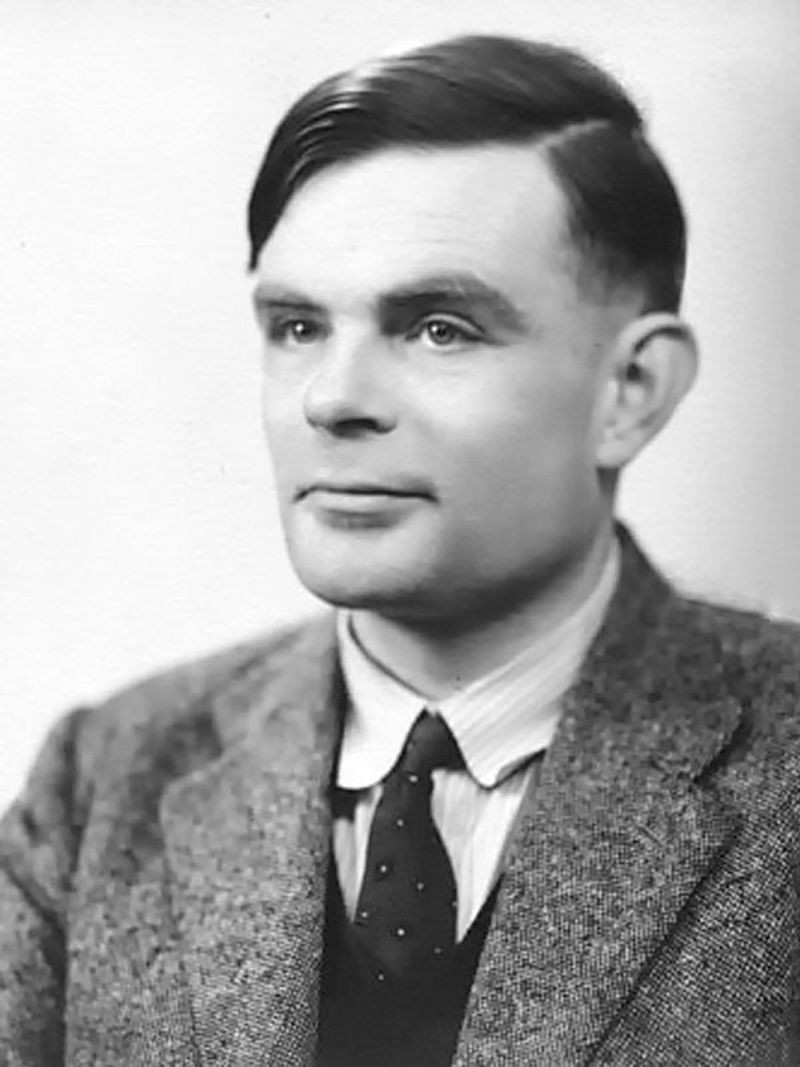
\includegraphics[width=0.85\textwidth]{../book/_static/external_images/alan_turing_1951.jpg}\\[0.3em]
      {\tiny\textit{Source: Elliott \& Fry (1951), public domain}}
    \end{column}
  \end{columns}
\end{frame}

\begin{frame}{The formal birth: the Dartmouth workshop (1956)}
  AI formally crystallized as a research field in \textbf{1956}, when John McCarthy organized the \textbf{Dartmouth workshop}, a multi-week gathering that brought together the leading researchers of the time.

  McCarthy put forward a very ambitious conjecture: every aspect of learning or intelligence could be described so precisely that a machine could simulate it.

  For the following decades, most experts believed human-level intelligence would be reached by hand-coding a massive set of \textbf{explicit logical rules}. This approach, known as \textbf{symbolic AI}, peaked with \textbf{expert systems} in the 1980s.

  \ejemplo{a typical 1980s medical expert system contained thousands of rules of the form ``if fever and cough and chest pain, then suspect pneumonia'', hand-written by doctors and programmers.}
\end{frame}

\begin{frame}{The Perceptron and the ``AI winters''}
  \begin{columns}
    \begin{column}{0.6\textwidth}
      In \textbf{1958}, Frank Rosenblatt created the \textbf{Perceptron}, the first artificial-neuron model able to \textit{learn} by adjusting its own parameters from examples, instead of having them hand-programmed.

      AI's history has not been steady progress, but a sequence of cycles of extreme enthusiasm followed by disillusionment and funding cuts, known as \textbf{``AI winters''}:
      \begin{itemize}
        \item \textbf{First winter} (1970s): it was discovered that the simple Perceptron could not solve problems that were not linearly separable.
        \item \textbf{Second winter} (1990s): expert systems turned out to be expensive to maintain, hard to scale, and limited to very narrow domains.
      \end{itemize}
    \end{column}
    \begin{column}{0.35\textwidth}
      \centering
      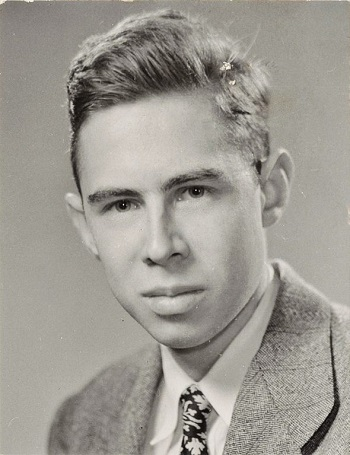
\includegraphics[width=0.88\textwidth]{../book/_static/external_images/frank_rosenblatt.jpg}\\
      \fuente{Heinz Nixdorf MuseumsForum, CC BY-SA 4.0}
    \end{column}
  \end{columns}
\end{frame}

\begin{frame}{Full timeline}
  Machine learning truly took off in the 1990s, driven by faster hardware and the availability of large amounts of data. Unlike symbolic AI ---suited to logical problems such as chess---, ML made it possible to tackle ``fuzzy'' problems such as speech recognition or image classification.
  \begin{center}
    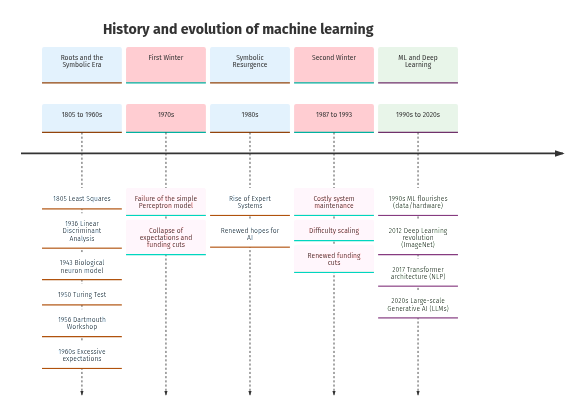
\includegraphics[width=0.48\textwidth]{../book/_static/generated/diagrams_pdf/en/00_fundamentals_01_history_evolution_01.png}
  \end{center}
\end{frame}

\begin{frame}{The rise of \textit{Deep Learning} (2010-2016)}
  \textbf{Deep Learning} is a specialized branch of ML that learns \textbf{successive layered representations}: each layer of the neural network receives the output of the previous one and extracts patterns that are increasingly useful for the task.

  The turning point came in \textbf{2012}, when Geoffrey Hinton's team won the \textbf{ImageNet} image-classification challenge by a wide margin, using a deep neural network instead of the traditional statistical methods that had dominated until then.

  During this period, the \textbf{MNIST} dataset (handwritten digits 0-9) became the quintessential benchmark for comparing classification algorithms.
  \begin{center}
    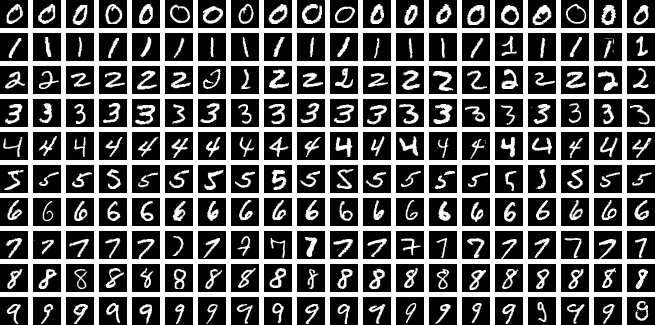
\includegraphics[width=0.3\textwidth]{../book/_static/external_images/mnist_dataset_example.png}\\
    \fuente{Suvanjanprasai (2024), Wikimedia Commons, CC BY-SA 4.0}
  \end{center}
\end{frame}

\begin{frame}{The LLM era (2017-today)}
  Starting in \textbf{2017}, the \textbf{Transformer} architecture ---which uses an ``attention'' mechanism to process text sequences without recurrent layers--- unleashed a revolution in natural language processing.

  This enabled training \textbf{foundation models} through \textbf{self-supervised learning} on enormous amounts of internet text: the model learns by predicting words it hides from itself, without needing human-created labels.

  The current era is marked by \textbf{Generative AI} (such as ChatGPT or Gemini), which scales the technology to billions of parameters and allows it not only to classify data, but to \textbf{generate} new content: text, images, code, or audio, thanks to \textbf{LLMs} (\textit{Large Language Models}).
\end{frame}

% ============================================================
\section{1.2 Fundamental concepts}

\begin{frame}{Data, features, and labels}
  The success of any ML system depends on how the information is represented. Consider a typical table:
  \begin{center}
    \small
    \begin{tabular}{lcccc}
      \toprule
      Sample & Feature 1 & Feature 2 & Feature 3 & Label \\
      \midrule
      1 & 25 & 70 & 175 & Cat \\
      2 & 8 & 4 & 90 & Cat \\
      3 & 35 & 80 & 180 & Dog \\
      \bottomrule
    \end{tabular}
  \end{center}
  \begin{itemize}
    \item \textbf{Sample}: the basic unit of information (one row of the table), also called an instance or data point.
    \item \textbf{Features}: the attributes describing each sample (the input columns).
    \item \textbf{Label}: the correct answer associated with each sample; the set of all labels makes up the \textbf{``ground truth''}.
  \end{itemize}
\end{frame}

\begin{frame}{Overfitting vs. underfitting}
  The fundamental problem in machine learning is the tension between fitting the model to known data and its ability to work well on new data:
  \begin{itemize}
    \item \textbf{Underfitting}: the model is too simple to capture the real pattern in the data. Both training and validation error are high.
    \item \textbf{Overfitting}: the model is too complex and ends up memorizing the noise in the training data. Training error is very low, but validation error is high.
    \item The goal is to find the \textbf{bias-variance} trade-off: low bias (the model doesn't oversimplify) and low variance (the model isn't overly sensitive to the specific training data).
  \end{itemize}
  \ejemplo{\footnotesize it's like studying for an exam by memorizing the exact answers of one mock test (overfitting) instead of understanding the topic: you'll fail as soon as the questions change a little.}
  \begin{center}
    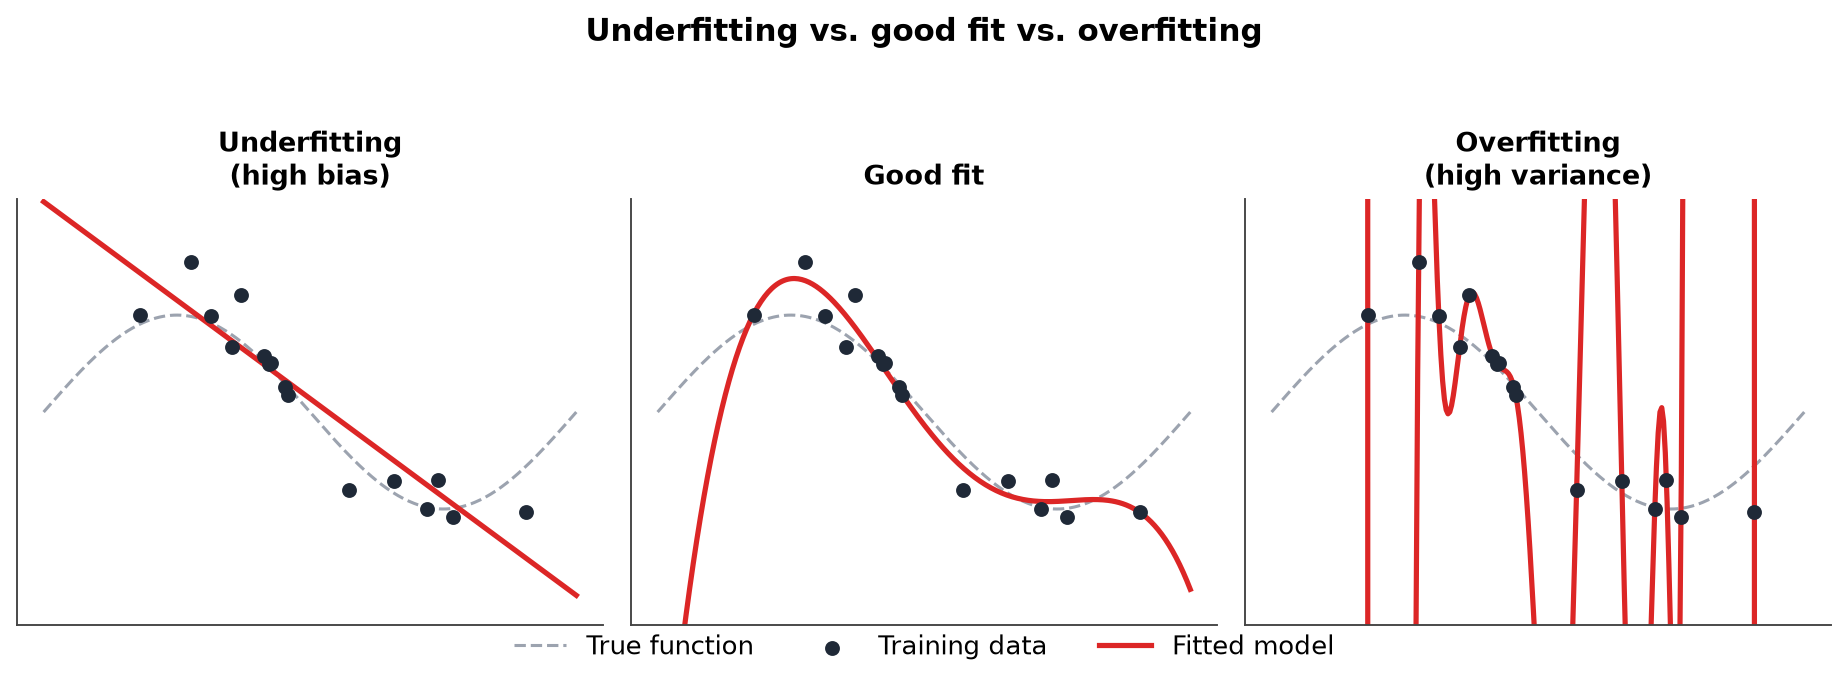
\includegraphics[width=0.34\textwidth]{../book/_static/generated/figures/en/overfitting_underfitting.png}
  \end{center}
\end{frame}

\begin{frame}{$K$-fold cross-validation}
  To measure generalization reliably, it is not enough to evaluate the model on the same data it was trained on. The standard practice is to split the data into three sets:
  \begin{itemize}
    \item \textbf{Training}: to fit the model's weights.
    \item \textbf{Validation}: to choose hyperparameters and compare models.
    \item \textbf{Test}: reserved for a final, unbiased evaluation.
  \end{itemize}
  When data is scarce, $K$-fold cross-validation makes better use of the information: the data is split into $K$ parts, the model is trained $K$ times (each time using a different part as validation), and the final metric is the \textbf{average} of the $K$ results. \textbf{Stratification} ensures each partition keeps the same class proportions as the original dataset.
  \begin{center}
    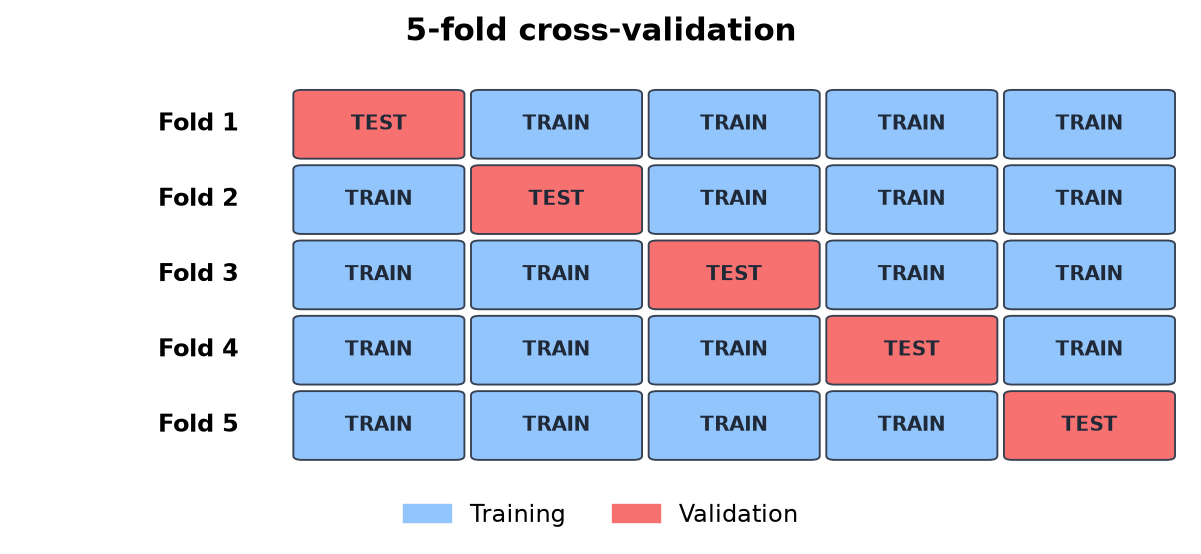
\includegraphics[width=0.4\textwidth]{../book/_static/generated/figures/en/kfold_cross_validation.png}
  \end{center}
\end{frame}

\begin{frame}{Confusion matrix}
  To evaluate a classifier we use a table called the \textbf{confusion matrix}, which compares the true labels with the model's predictions:
  \begin{columns}
    \begin{column}{0.5\textwidth}
      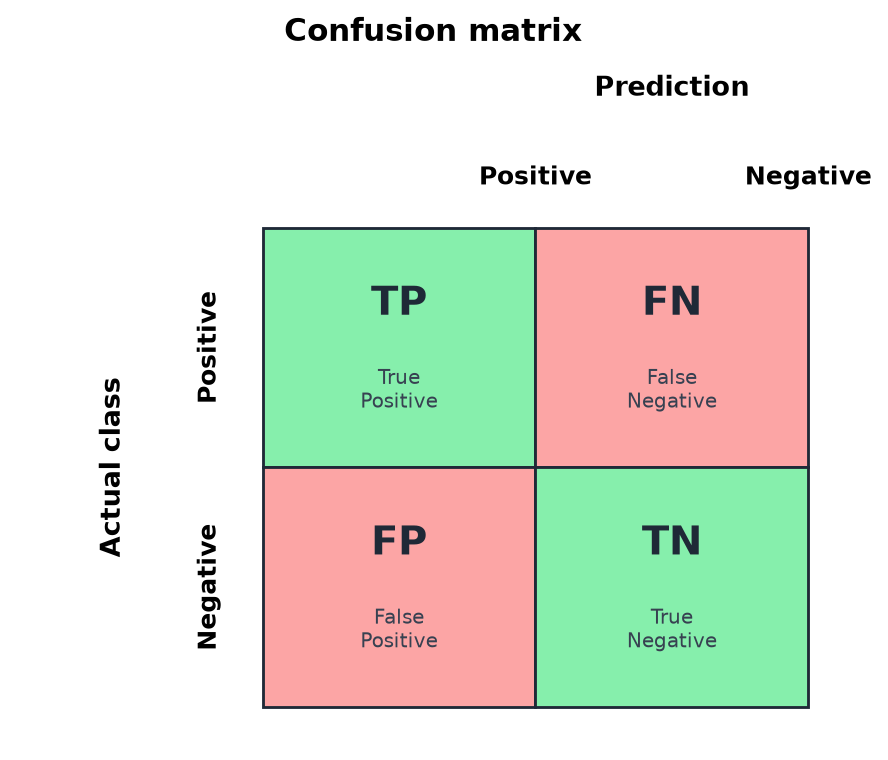
\includegraphics[width=0.6\textwidth]{../book/_static/generated/figures/en/confusion_matrix.png}
    \end{column}
    \begin{column}{0.5\textwidth}
      \small
      \begin{itemize}
        \item \textbf{TP} (true positive): a correct positive.
        \item \textbf{TN} (true negative): a correct negative.
        \item \textbf{FP} (false positive): a ``false alarm'' (type I error).
        \item \textbf{FN} (false negative): a ``miss'' (type II error).
      \end{itemize}
    \end{column}
  \end{columns}
  \ejemplo{\footnotesize in a medical diagnosis, a false negative (telling a sick person ``healthy'') is usually far more serious than a false positive.}
\end{frame}

\begin{frame}{Metrics derived from the confusion matrix}
  \small
  \begin{itemize}
    \item \textbf{Accuracy}: the percentage of correct predictions overall. Can be misleading when classes are imbalanced.
    \item \textbf{Precision}: of everything the model predicted as positive, how much was actually correct?
    \item \textbf{Recall} (sensitivity): of all the real positives out there, how many did the model find?
    \item \textbf{F1}: combines precision and recall into a single number; useful when both matter equally.
    \item \textbf{AUC-ROC}: measures how well the model tells positives and negatives apart, without depending on a fixed threshold. 1.0 is perfect, 0.5 is equivalent to chance.
  \end{itemize}
  \ejemplo{if 90\% of emails aren't spam, a model that always says ``not spam'' would have 90\% accuracy without having learned anything useful: that's why precision and recall sometimes matter more than accuracy alone.}
\end{frame}

\begin{frame}{The ML \textit{pipeline}: 10 stages}
  Developing a machine learning project follows a universal workflow, from data collection to production deployment. It is an \textbf{iterative} process: the evaluation stage often forces a return to earlier stages (for example, collecting more data or tuning hyperparameters) before the project can be considered finished.
  \begin{columns}
    \begin{column}{0.42\textwidth}
      \footnotesize
      \begin{enumerate}
        \item Data collection
        \item Exploration and cleaning
        \item Feature engineering
        \item Train/test split
        \item Model selection
        \item Training
      \end{enumerate}
    \end{column}
    \begin{column}{0.42\textwidth}
      \footnotesize
      \begin{enumerate}
        \setcounter{enumi}{6}
        \item Evaluation
        \item Hyperparameter tuning
        \item Final evaluation
        \item Deployment (and continuous monitoring)
      \end{enumerate}
    \end{column}
  \end{columns}
  \begin{center}
    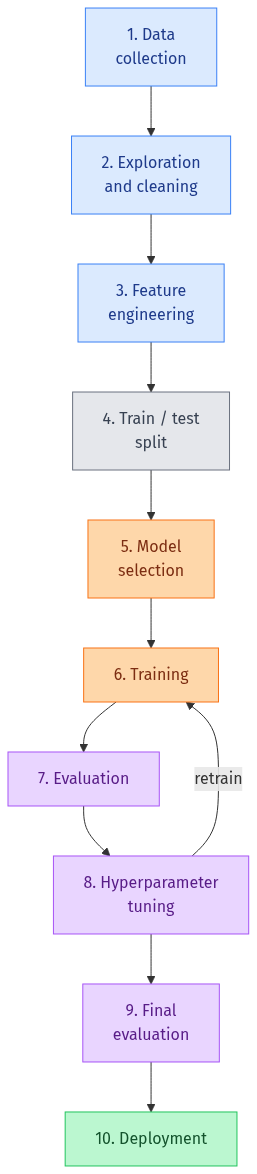
\includegraphics[height=0.26\textheight]{../book/_static/generated/diagrams_pdf/en/00_fundamentals_02_fundamental_concepts_01.png}
  \end{center}
\end{frame}

% ============================================================
\begin{frame}{Chapter summary}
  \small
  \begin{itemize}
    \item Machine learning was born from a very simple question: \textbf{can machines learn?}
    \item Its history has not been linear: it has gone through cycles of hype and ``winters'' of disillusionment and funding cuts.
    \item The current state of the art is \textbf{deep learning} and \textbf{LLMs}, made possible by more data, better hardware, and more efficient algorithms.
    \item \textbf{Sample}, \textbf{feature}, and \textbf{label} are the basic building blocks of any dataset.
    \item \textbf{Overfitting}/\textbf{underfitting} and \textbf{cross-validation} are the tools for knowing whether a model generalizes well.
    \item The \textbf{confusion matrix} and its derived metrics let you pick the right success measure for the problem at hand.
    \item The ML \textbf{\textit{pipeline}} organizes the whole process into 10 iterative stages, from data to deployment.
  \end{itemize}
\end{frame}

% ============================================================
\begin{frame}{License of these slides}
  \begin{center}
    This material is distributed under a\\[0.3em]
    {\large\textbf{\textcolor{usalred}{Creative Commons Attribution-NonCommercial 4.0}}}\\[0.2em]
    {\footnotesize (CC BY-NC 4.0)}
  \end{center}
  \vspace{0.3em}
  \small
  \begin{columns}[t]
    \begin{column}{0.47\textwidth}
      \textbf{\textcolor{usalred}{You are free to:}}
      \begin{itemize}
        \item \textbf{Share}: copy and redistribute the material in any medium or format.
        \item \textbf{Adapt}: remix, transform and build upon the material.
      \end{itemize}
      {\footnotesize For example: use them in class, upload them to a virtual campus, translate them or reuse a figure in your own notes.}
    \end{column}
    \begin{column}{0.47\textwidth}
      \textbf{\textcolor{usalred}{Under the following terms:}}
      \begin{itemize}
        \item \textbf{Attribution (BY)}: you must credit the author, link to the license and indicate if changes were made.
        \item \textbf{NonCommercial (NC)}: you may not use the material for commercial purposes.
      \end{itemize}
      {\footnotesize You may not add restrictions that legally prevent others from doing anything the license permits.}
    \end{column}
  \end{columns}
  \vspace{0.4em}
  \begin{center}
    {\footnotesize\texttt{creativecommons.org/licenses/by-nc/4.0/}}
  \end{center}
\end{frame}

\titleslide

\end{document}
